
\begin{frame}
  \frametitle{Nuclear Forensics Investigations}
  \begin{minipage}[t]{0.5\textwidth}
    \textbf{Post-detonation}
    \begin{itemize}
      \item Collection: debris, swipe samples
      \item Characterization: rapid analysis of isotope ratios
      \item Goals
      \begin{itemize}
        \item Inverse problem: reconstruct weapon design/yield
        \item Safety: informing disaster response
      \end{itemize}
      \item Data evaluation
    \end{itemize}
  \end{minipage}%
  \pause
  \begin{minipage}[t]{0.5\textwidth}
    \textbf{Pre-detonation}
    \begin{itemize}
      \item Collection: depends on intercepted material
      \item \boxalert{Characterization:} non-destructive and destructive
      \item Goals:
      \begin{itemize}
        \item \boxalert{Inverse problem:} material chain of custody
        \item Safety: material handling and security
      \end{itemize}
      \item \boxalert{Data evaluation}
    \end{itemize}
  \end{minipage}
\end{frame}


\begin{frame}
  \frametitle{Nuclear Forensics as an Inverse Problem}
  \begin{minipage}[t]{0.5\textwidth}
  Use Bayes' Framework:\\
  $ P(M|D) = \frac{P(D|M)P(M)}{P(D)} $
  \end{minipage}%
  \begin{minipage}[t]{0.5\textwidth}
    M : \textbf{M}odel parameters\\
    D : Measured \textbf{D}ata
  \end{minipage}
  \vfill
  \vfill
  \begin{table}
    \centering
    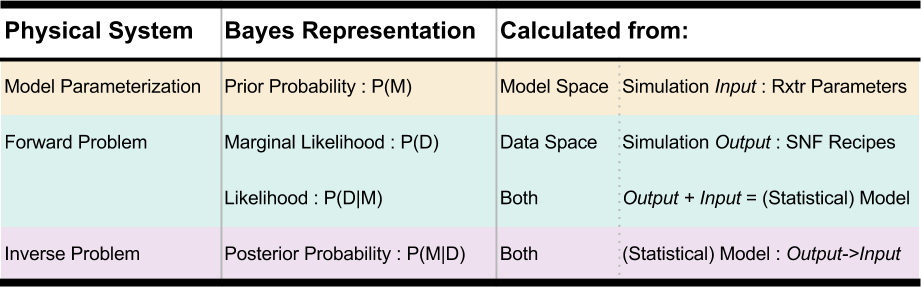
\includegraphics[width=\textwidth]{./figures/InverseIntro.png}
    \caption{Mapping the study of a physical system its Bayesian representation}
  \end{table}
\end{frame}

